\documentclass[12pt]{article}
\usepackage[a4paper, portrait, margin=1cm, right=1cm]{geometry}
\usepackage{fontspec}
\usepackage{graphicx}
\usepackage[fleqn]{amsmath}
\usepackage{setspace}

\graphicspath{./graphics/}
\setmainfont[Ligatures=TeX]{Linux Libertine}

\title{Информационные технологии. Лекция 06}
\author{Студент группы 2305 Макурин Александр}
\date{27 марта 2023}
\begin{document}
\maketitle
\[
    t_\text{пр.р.} = 2 \alpha t_\alpha + \beta t_\beta + \varepsilon
\]

$t_\text{пр.р.}$ — общее время принятия решения. $\alpha$, $\beta$ — коэффициенты сложности. $t_\alpha$ — время доставки сигнала. $t_\beta$ — время принятия решения. $\varepsilon$ — время работы манипулятора (механики).

Можно представить работу КФС делиберативной архитектуры в виде следующей схемы:

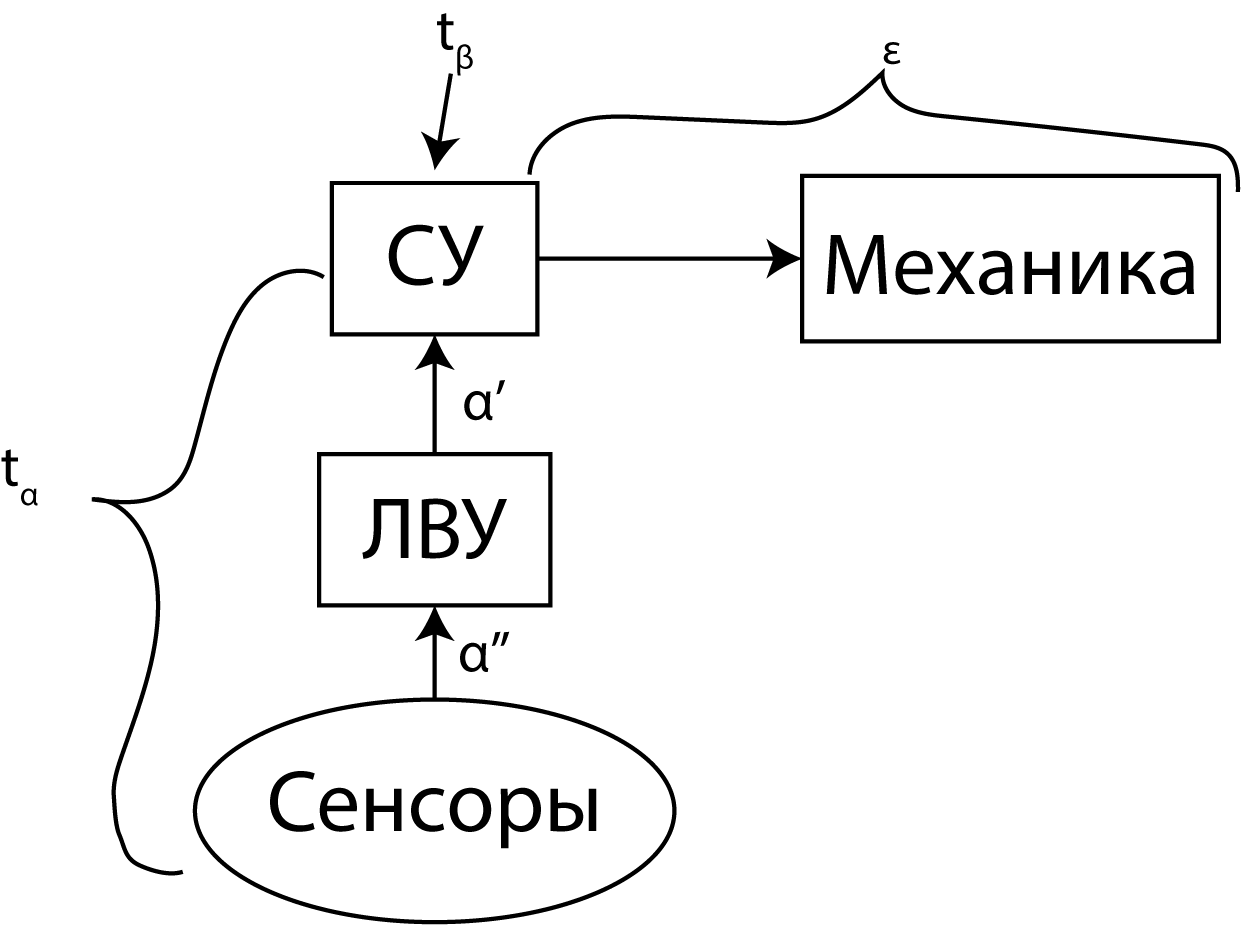
\includegraphics{graphics/Сенсоры-ЛВУ-СУ-Механика.png}

ЛВУ — локальное вычислительное устройство — на нём происходит обработка данных с сенсоров. СУ — система управления.

\[
    t_\alpha = \alpha' t_{\text{ЛВУ}_\alpha} + \alpha'' t_{\text{СУ}_\alpha}
\]
\[
    t_\beta = \alpha' t_{\text{ЛВУ}_\beta} + \alpha'' t_{\text{СУ}_\beta}
\]

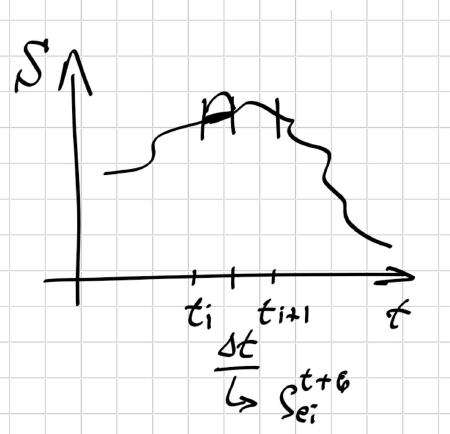
\includegraphics[width=0.3\textwidth]{graphics/pic01.png}

При $\Delta t = \text{const}$ возможен следующий переход (от верхнего к нижнему): \\
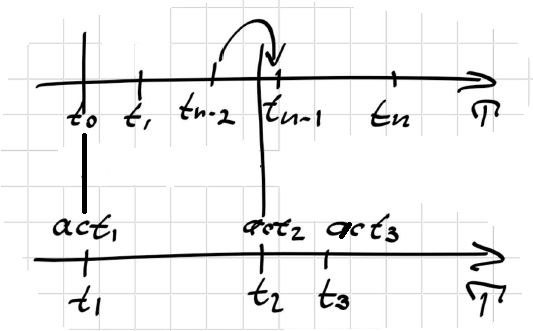
\includegraphics[width=0.5\textwidth]{graphics/pic02.png}

В Gazebo время идёт как на верхнем графике: $\Delta t = \text{const}$.

На нижнем графике, очевидно, $\Delta t \neq \text{const}$. Такой случай называется дискретно-событийным моделированием.

Когда $\lim t_\text{пр.р.} < \Delta t$ — всё хорошо. Но в идеальном мире $\Delta t \rightarrow 0 \ (\overline{\Delta t} \rightarrow 0)$.

Возможен обратный переход от дискретно-событийного моделирования к дискретному по времени посредством разделения участка между двумя событиями на более мелкие:

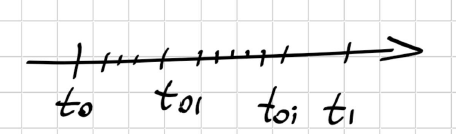
\includegraphics[width=0.5\textwidth]{graphics/pic03.png}

\[
    \overline{\Delta t} = \text{const},\ \overline{\Delta t} < \Delta t,\ \Delta t = t_1 - t_0
\]

$\Delta t$ нужно выбрать максимально малым.

В реальности: $\lim t_{\text{пр.р.}} \geq \Delta t$.

\[
    \widetilde{f}(S^t, x_i, \{S^{t - 1}\}) = \overline{f}(S^{t + \varepsilon}...) \rightarrow S^t
\]

Необходимо разработать систему, стабилизирующуюся ещё на ЛВУ — т. е. способную принимать локальные решения:

\[
    E{\overline{f}^{t + \varepsilon_1},..., \overline{f}^{t + \varepsilon_k}} = ES^t
\]

$E$ — математическое ожидание.

Гипотеза: можно взять такую $\Delta t$, что поведение состояния системы на отрезке можно будет представить линейной функцией.

Фильтр Калмана:
\begin{itemize}
    \item Предсказание: \\
          1. Локализация: $S^{t-} = \alpha_1 S^{t-1} + \alpha_2 U^{t - 1}$ \\
          2. GPS: $p^{t-} = \beta p^{t - 1} \beta^T + \Omega$ \\
          $S^{t-}$ — прогнозируемое состояние системы. $p^{t-}$ — анализ состояния. $\alpha_1, \alpha_2, \beta$ — гиперпараметры (прошлых состояний среды и внешних воздействий). $\Omega$ — белый Гауссовский шум.
    \item Корректировка: \\
          3. $K^t = p^{t-} H^T(Hp^{t-}H^T + R)^{-1}$ \\
          4. $S^t = S^{t-} + K^t(A^t - H S_t^-)$ \\
          5. $p^t = (I - K^tH)p^{t-}$ \\
          $H$ — матрица отношений измеренного и реального состояний $\dfrac{S}{p}$. Чем меньше, тем лучше. $R$ — шум (влияние одного параметра на другие). Позволяет объединить данные с разных датчиков. $A^t$ — внешние данные. Если $A^t - HS_t^- = 0$, то состояние зависит только от внутреннего состояния системы. $|H| = |S|$.

          Пример $H$: \\
          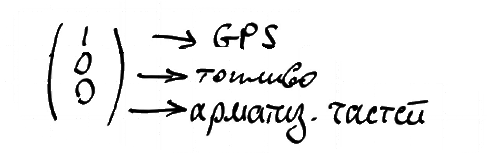
\includegraphics[width=0.5\textwidth]{graphics/pic04.png}

          Корреляция — зависимость одного столбца от другого.
\end{itemize}

\[
    f(S^t, x, \{S^{t - 1}\})
\]

\[
    \overline{t_\text{пр.р.}} = \sum t_\text{пр.р.}^\text{дат.} + \varepsilon
\]
\[
    \overline{t_\text{пр.р.}} \rightarrow min t_\text{пр.р.}^\text{дат.}
\]

\[
    S_{e_i} = \cup I^\text{дат.} + \nu
\]

\[
    S_{e_i}^\text{дат.1} \cap S_{e_i}^\text{дат.2} = \emptyset \Rightarrow \text{датчики друг с другом не контактируют}
\]

$\beta t_\beta$ можно разбить на $t_{est}$ (время интеллектуального анализа данных) и $t_f$ (время формирования плана).

\end{document}